% generated by scripts/pkl_to_latex.py
% source PKL : uscan_v1_L8_Ne8_t1_mode-uniform_nmin2_solver-gcg_full_restarts8_iter200_kmax4_tol1em09_U1to20_N20-d03a74da789e.pkl
% scan type  : uscan
% state      : gs
% requires   : \usepackage{pgfplots} \pgfplotsset{compat=1.18}
% colours match the matplotlib PDF (tab10 cycle)
\definecolor{gmeC0}{HTML}{1F77B4}
\definecolor{gmeC1}{HTML}{FF7F0E}
\definecolor{gmeC2}{HTML}{2CA02C}
\definecolor{gmeC3}{HTML}{D62728}
\definecolor{gmeC4}{HTML}{9467BD}
\definecolor{gmeC5}{HTML}{8C564B}
\definecolor{gmeC6}{HTML}{E377C2}
\definecolor{gmeC7}{HTML}{17BECF}

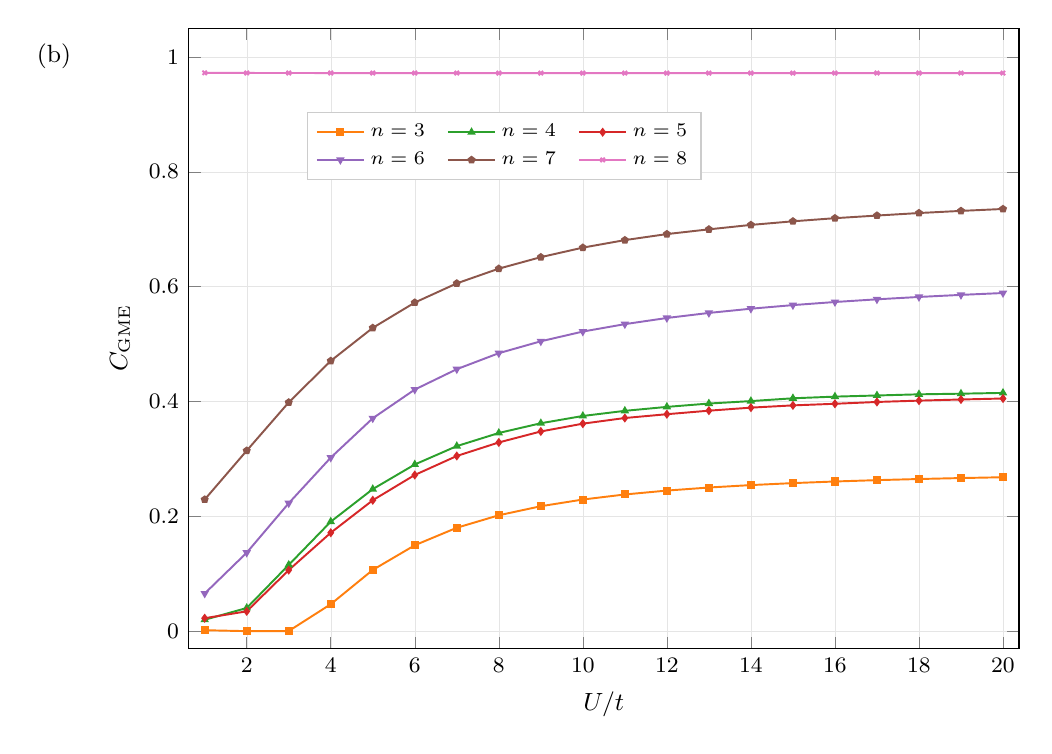
\begin{tikzpicture}
  \begin{axis}[
    width=\columnwidth,
    height=0.78\columnwidth,
    xlabel={$U/t$},
    ylabel={$C_{\mathrm{GME}}$},
    grid=both,
    grid style={line width=.1pt, draw=gray!20},
    tick label style={font=\footnotesize\rmfamily, /pgf/number format/fixed},
    label style={font=\small\rmfamily},
    scaled ticks=false,
    legend style={font=\scriptsize\rmfamily, draw=gray!40, at={(0.5,1.03)}, anchor=south, /tikz/every even column/.append style={column sep=6pt}},
    legend cell align={left},
    legend columns=3,
    ymin=-0.03,
    ymax=1.05,
    xmin=0.62,
    xmax=20.38,
    legend style={at={(0.380,0.810)}, anchor=center, fill=white},
    after end axis/.append code={\node[anchor=east, font=\small\rmfamily] at (axis description cs:-0.13,0.954) {(b)};},
  ]
    \addplot[color=gmeC1, mark=square*, mark size=1.1pt, line width=0.7pt] coordinates {
        (1,0.001654) (2,0.000044) (3,0.000267) (4,0.046975)
        (5,0.106664) (6,0.149618) (7,0.180102) (8,0.201846)
        (9,0.217602) (10,0.229253) (11,0.238052) (12,0.244832)
        (13,0.250153) (14,0.2544) (15,0.257839) (16,0.260662)
        (17,0.263006) (18,0.264974) (19,0.266641) (20,0.268065)
    };
    \addlegendentry{$n=3$}
    \addplot[color=gmeC2, mark=triangle*, mark size=1.1pt, line width=0.7pt] coordinates {
        (1,0.019878) (2,0.040367) (3,0.115422) (4,0.190681)
        (5,0.247387) (6,0.290277) (7,0.322264) (8,0.345138)
        (9,0.362087) (10,0.374752) (11,0.383696) (12,0.390574)
        (13,0.396403) (14,0.400666) (15,0.405558) (16,0.408454)
        (17,0.410431) (18,0.412454) (19,0.413562) (20,0.414928)
    };
    \addlegendentry{$n=4$}
    \addplot[color=gmeC3, mark=diamond*, mark size=1.1pt, line width=0.7pt] coordinates {
        (1,0.022574) (2,0.034548) (3,0.106354) (4,0.171385)
        (5,0.228007) (6,0.272007) (7,0.305072) (8,0.328669)
        (9,0.347784) (10,0.36136) (11,0.371204) (12,0.377835)
        (13,0.383977) (14,0.389274) (15,0.393186) (16,0.395985)
        (17,0.39916) (18,0.401473) (19,0.403454) (20,0.405168)
    };
    \addlegendentry{$n=5$}
    \addplot[color=gmeC4, mark=triangle*, mark size=1.1pt, mark options={rotate=180}, line width=0.7pt] coordinates {
        (1,0.0656) (2,0.136722) (3,0.222841) (4,0.30224)
        (5,0.370771) (6,0.420742) (7,0.456253) (8,0.484101)
        (9,0.504819) (10,0.521759) (11,0.534672) (12,0.545395)
        (13,0.55418) (14,0.561558) (15,0.567815) (16,0.573218)
        (17,0.577909) (18,0.58201) (19,0.585636) (20,0.588864)
    };
    \addlegendentry{$n=6$}
    \addplot[color=gmeC5, mark=pentagon*, mark size=1.1pt, line width=0.7pt] coordinates {
        (1,0.229283) (2,0.314356) (3,0.39842) (4,0.470714)
        (5,0.528206) (6,0.572269) (7,0.605691) (8,0.631318)
        (9,0.651337) (10,0.667933) (11,0.680997) (12,0.691507)
        (13,0.699756) (14,0.707466) (15,0.713749) (16,0.719196)
        (17,0.723774) (18,0.728158) (19,0.731886) (20,0.735217)
    };
    \addlegendentry{$n=7$}
    \addplot[color=gmeC6, mark=x, mark size=1.1pt, line width=0.7pt] coordinates {
        (1,0.972294) (2,0.97209) (3,0.971991) (4,0.971943)
        (5,0.971918) (6,0.971905) (7,0.971898) (8,0.971894)
        (9,0.971891) (10,0.97189) (11,0.971889) (12,0.971888)
        (13,0.971888) (14,0.971887) (15,0.971887) (16,0.971887)
        (17,0.971887) (18,0.971887) (19,0.971887) (20,0.971887)
    };
    \addlegendentry{$n=8$}
  \end{axis}
\end{tikzpicture}
